\chapter{Social Connectedness Index}
\taskID{44}{Social Connectedness Index from Facebook}

\section{Introduction}
The \emph{Social Connectedness Index} (SCI) measures the strength of the connection between pairs of geographical regions \cite{MetaForGood}. Firstly introduced in 2018 to analyze connectedness across US counties \cite{bailey2018social}, it is based on an anonymized snapshot of active Facebook users and their friendship networks. \\
Specifically, the SCI measures the relative probability that two individuals across two locations are friends on Facebook. The SCI between two locations $i$ and $j$ can be formalized as:
\begin{equation}
    SCI(i, j) = \frac{FB-connections(i, j)}{FB-users(i)*FB-users(j)} \quad \text{,}
\label{eq:SCI}
\end{equation}
where $FB-users(i)$ and $FB-users(j)$ are the number of Facebook users in location $i$ and $j$ according to their profile, and $FB-connections(i, j)$ represents the number of Facebook friendship connections between those two regions. The denominator of \eqref{eq:SCI} is the total number of possible connections, i.e. the possible pairs of users \footnote{If $i$ and $j$ are the same, the denominator is adjusted as $FB-users(i)*(FB-users(j)-1)$ since users cannot be friends with themselves.}. \\
The data have been collected and processed following the methodology described in \cite{MetaForGood}. %Each user is assigned to a location according to the information available on Facebook (e.g. the city in the profile), and the information about devices and connections. The obtained SCI is then rescaled into the interval between one and one billion, removing locations with limited observations.  Before rounding the index to the nearest integer, some noise is added such that no individual or relation can be identified from the data. Finally, SCI is the reduced average of friendship ties after 10 random draws among 99\% of active Facebook users. \\
The data analyzed in this report refers to a snapshot of the active Facebook users on October 13, 2021. This dataset should not be compared with older ones, since the SCI methodology has changed over time. \\
The geographic locations are obtained using the \textit{Database of Global
Administrative Areas} (GADM, version $2.8$) and the \textit{European Nomenclature of Territorial Units for Statistics} (NUTS 2016). European countries are divided into their NUTS3 regions (e.g. $110$ regions in Italy), while most other countries are usually divided into their GADM level 1 regions \footnote{Countries with a population less than 1 million are not divided.}. The United States, Canada, and some countries in South Asia are divided into their
GADM level 2 regions (e.g., US counties) due to their sizes. \\
The task is to build a - possibly weighted - network for each country. The output consists of two files: one for nodes, including latitude and longitude for each location, and one for edges list. 

\section{Methods and analysis}
The analysis leverages three R libraries: \texttt{geodata} \cite{geodata} (for GADM regions), \texttt{eurostat} \cite{eurostat} (for NUTS regions), and \texttt{tigris} \cite{tigris} (for USA counties). Briefly, the pipeline consists of associating each region to the corresponding country and level (e.g. GADM1, GADM2, ...), extracting the metadata of each node (latitude, longitude, name, ID), and creating the node table and the edge list. \\
The major limitation of this analysis regards the GADM version: the SCI data uses version 2.8 (released in 2015), while the oldest online available version is 3.6 (released in 2020). Version 2.8 should be available through the official GADM website \cite{GADM}, but no shapefile can currently be downloaded. Since the official log is under development, estimating what biases we are introducing using a different version is not trivial. The only observable consequence is that two countries (United Arab Emirates and Indonesia) were expected to have one more region each. 

\section{Comparisons}
All the obtained graphs are \emph{complete} (at least one friendship relation for each pair of regions of the same country) and \emph{undirected}. Thus, many of the classical network metrics are trivial. However, one can consider the \emph{weighted} version of the networks and base the comparisons out of that. \\ 
In particular, figure \ref{fig:meta} (left) shows four analytics implemented in the \texttt{igraph} R package and how they relate with each other and with the number of network nodes. The mean betweenness, clustering coefficient, and weighted distance are correlated with the number of nodes. The feature that exhibits the largest variability is the mean entropy of the networks, which measures the global diversity between the vertices based on the Shannon entropy of their incident edges. \\
Figure \ref{fig:meta} (right) analyses the full world network of social connectivity and investigates the relation between the haversine distance and the strength of such connectivity. As expected, there is a negative correlation between these two quantities: closer areas tend to have stronger connections. 


\begin{figure}[h]
    \centering
    \begin{minipage}{0.5\textwidth}
        \centering
        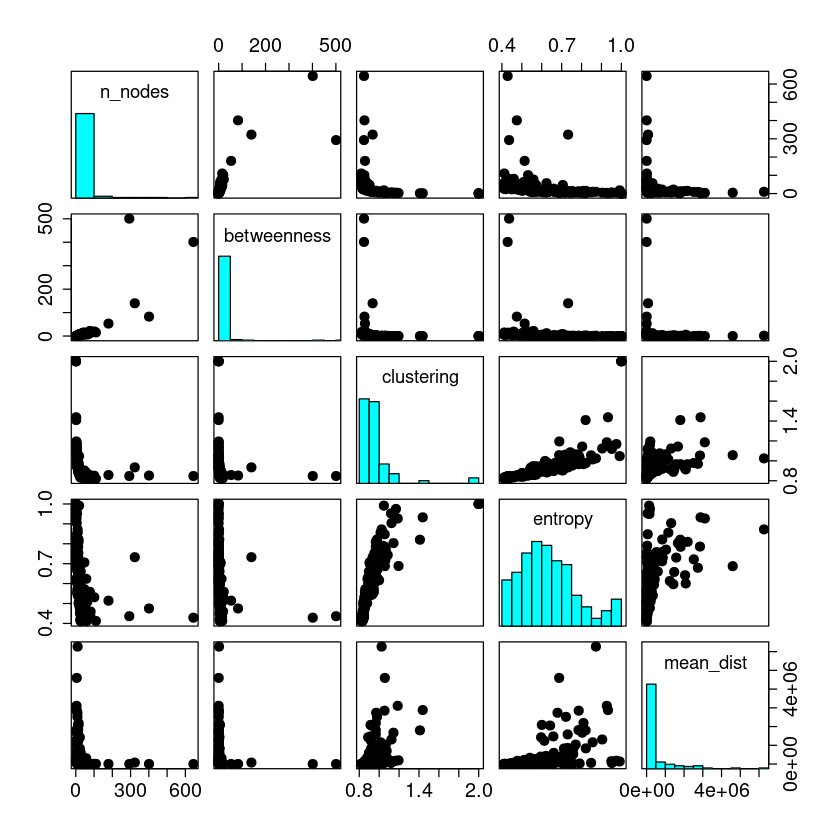
\includegraphics[width=\textwidth]{images/task44/dataNetworkComparison2.png}
        \label{fig:SCIcomparison}
    \end{minipage}\hfill
    \begin{minipage}{0.5\textwidth}
        \centering
        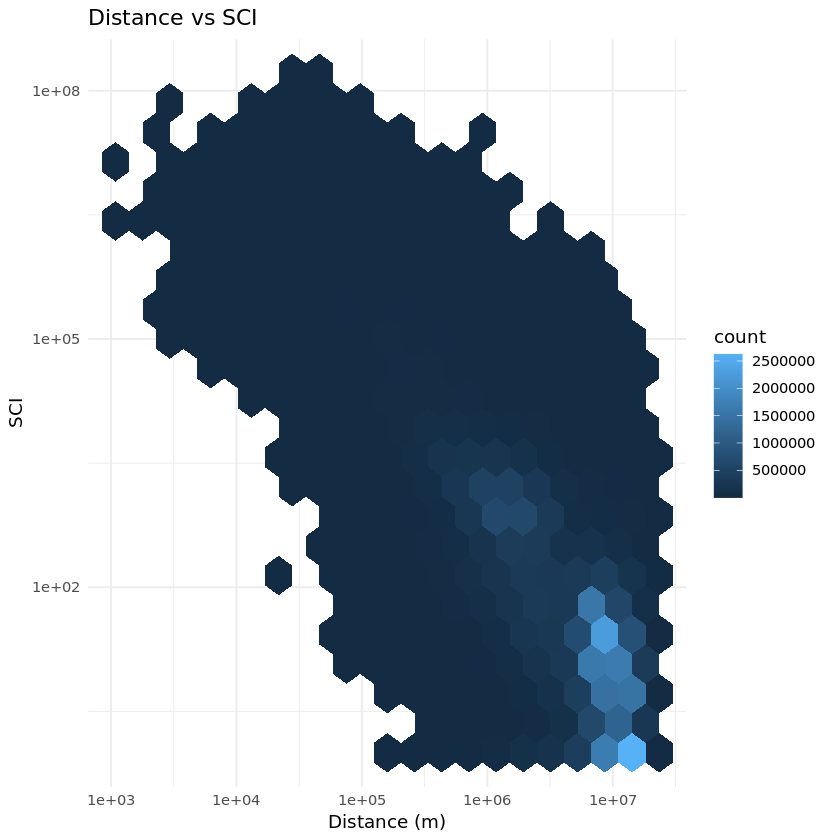
\includegraphics[width=\textwidth]{images/task44/dataDistanceSCI.png}
        \label{fig:SCIdistance}
    \end{minipage}
    \vspace{-1cm}
    \caption{(left) The pairwise relations between different metrics for the weighted networks. Each point is a country. (right) 2D histogram of the distribution of the SCI against the haversine distance.}
    \label{fig:meta}
\end{figure}

\newpage